\chapter{Experiments, Results and Discussions}
\label{chap:exp}
\framebox{REVIEW1}
\framebox{TODO:general introduction to the experiments}
In this chapter, we will use some experiment results to demonstrate the effectiveness of our method. Section \ref{sec:onsetnormexp} deals with the onset deviation problem highlighted in Section \ref{sec:normalize}. Section \ref{sec:paramselect} discusses how the various parameters in our system is decided, and their effect on the model and computing resource required. Section \ref{sec:turing} describes a Turing test to see if audience can or can't identify the difference between generated and human performances.


\section{Onset Deviation Normalization}
\label{sec:onsetnormexp}
\framebox{TODO:onset deviation problem review}
As mentioned in Section \ref{sec:normalize}, a bad normalization method will usually result in unreasonable high onset deviation, which will make the expressive performance sound very unnatural. To overcome this challenge, we proposed a automatic way to select the normalization parameter. In this section, we will evaluate the effectiveness of the method. 

We extract the onset deviation feature from a single performer's recording, using the four types of normalization method mentioned before and the automatic normalization method. The extracted onset deviations are shown in Fig. \ref{fig:normauto} to Fig.\ref{fig:norm3}. Each dotted line from left to right represents a phrase in the corpus. Each dot represents the onset deviation value of a note. The notes are spread uniformly  on the horizontal axis, which only shows the order of appearance, not the real time scale. First note that aligning the end of the last notes results in very large deviation in a few phrases. This is because performers tend to extend the last note in certain phrases to emphasize the end of a phrase or section. This kind of extension will cause the last notes onset to be far apart. So clearly this method is not a good way. Fig. \ref{fig:normauto} and Fig. \ref{fig:norm1} looks much similar, but the maximum and minimum value in Fig. \ref{fig:norm1} is more dramatic than those in Fig. \ref{fig:normauto}, which shows that the automatic normalization method can indeed find a better fit between the recorded phrase and the score. Another benefit of the automatic normalization is that the last note onset is not force aligned, which allows more free expression on the last note. In Fig. \ref{fig:norm1}, the end of a line, i.e. the last note, always goes back to zero; however in Fig. \ref{fig:normauto}, the end of a line can end in a wide range of values.

%\framebox{TODO:remove (quarter note) unit in figures} 
\begin{figure}[tp]
   \begin{center}
      %TODO:Fig.:Normalization Schemes
      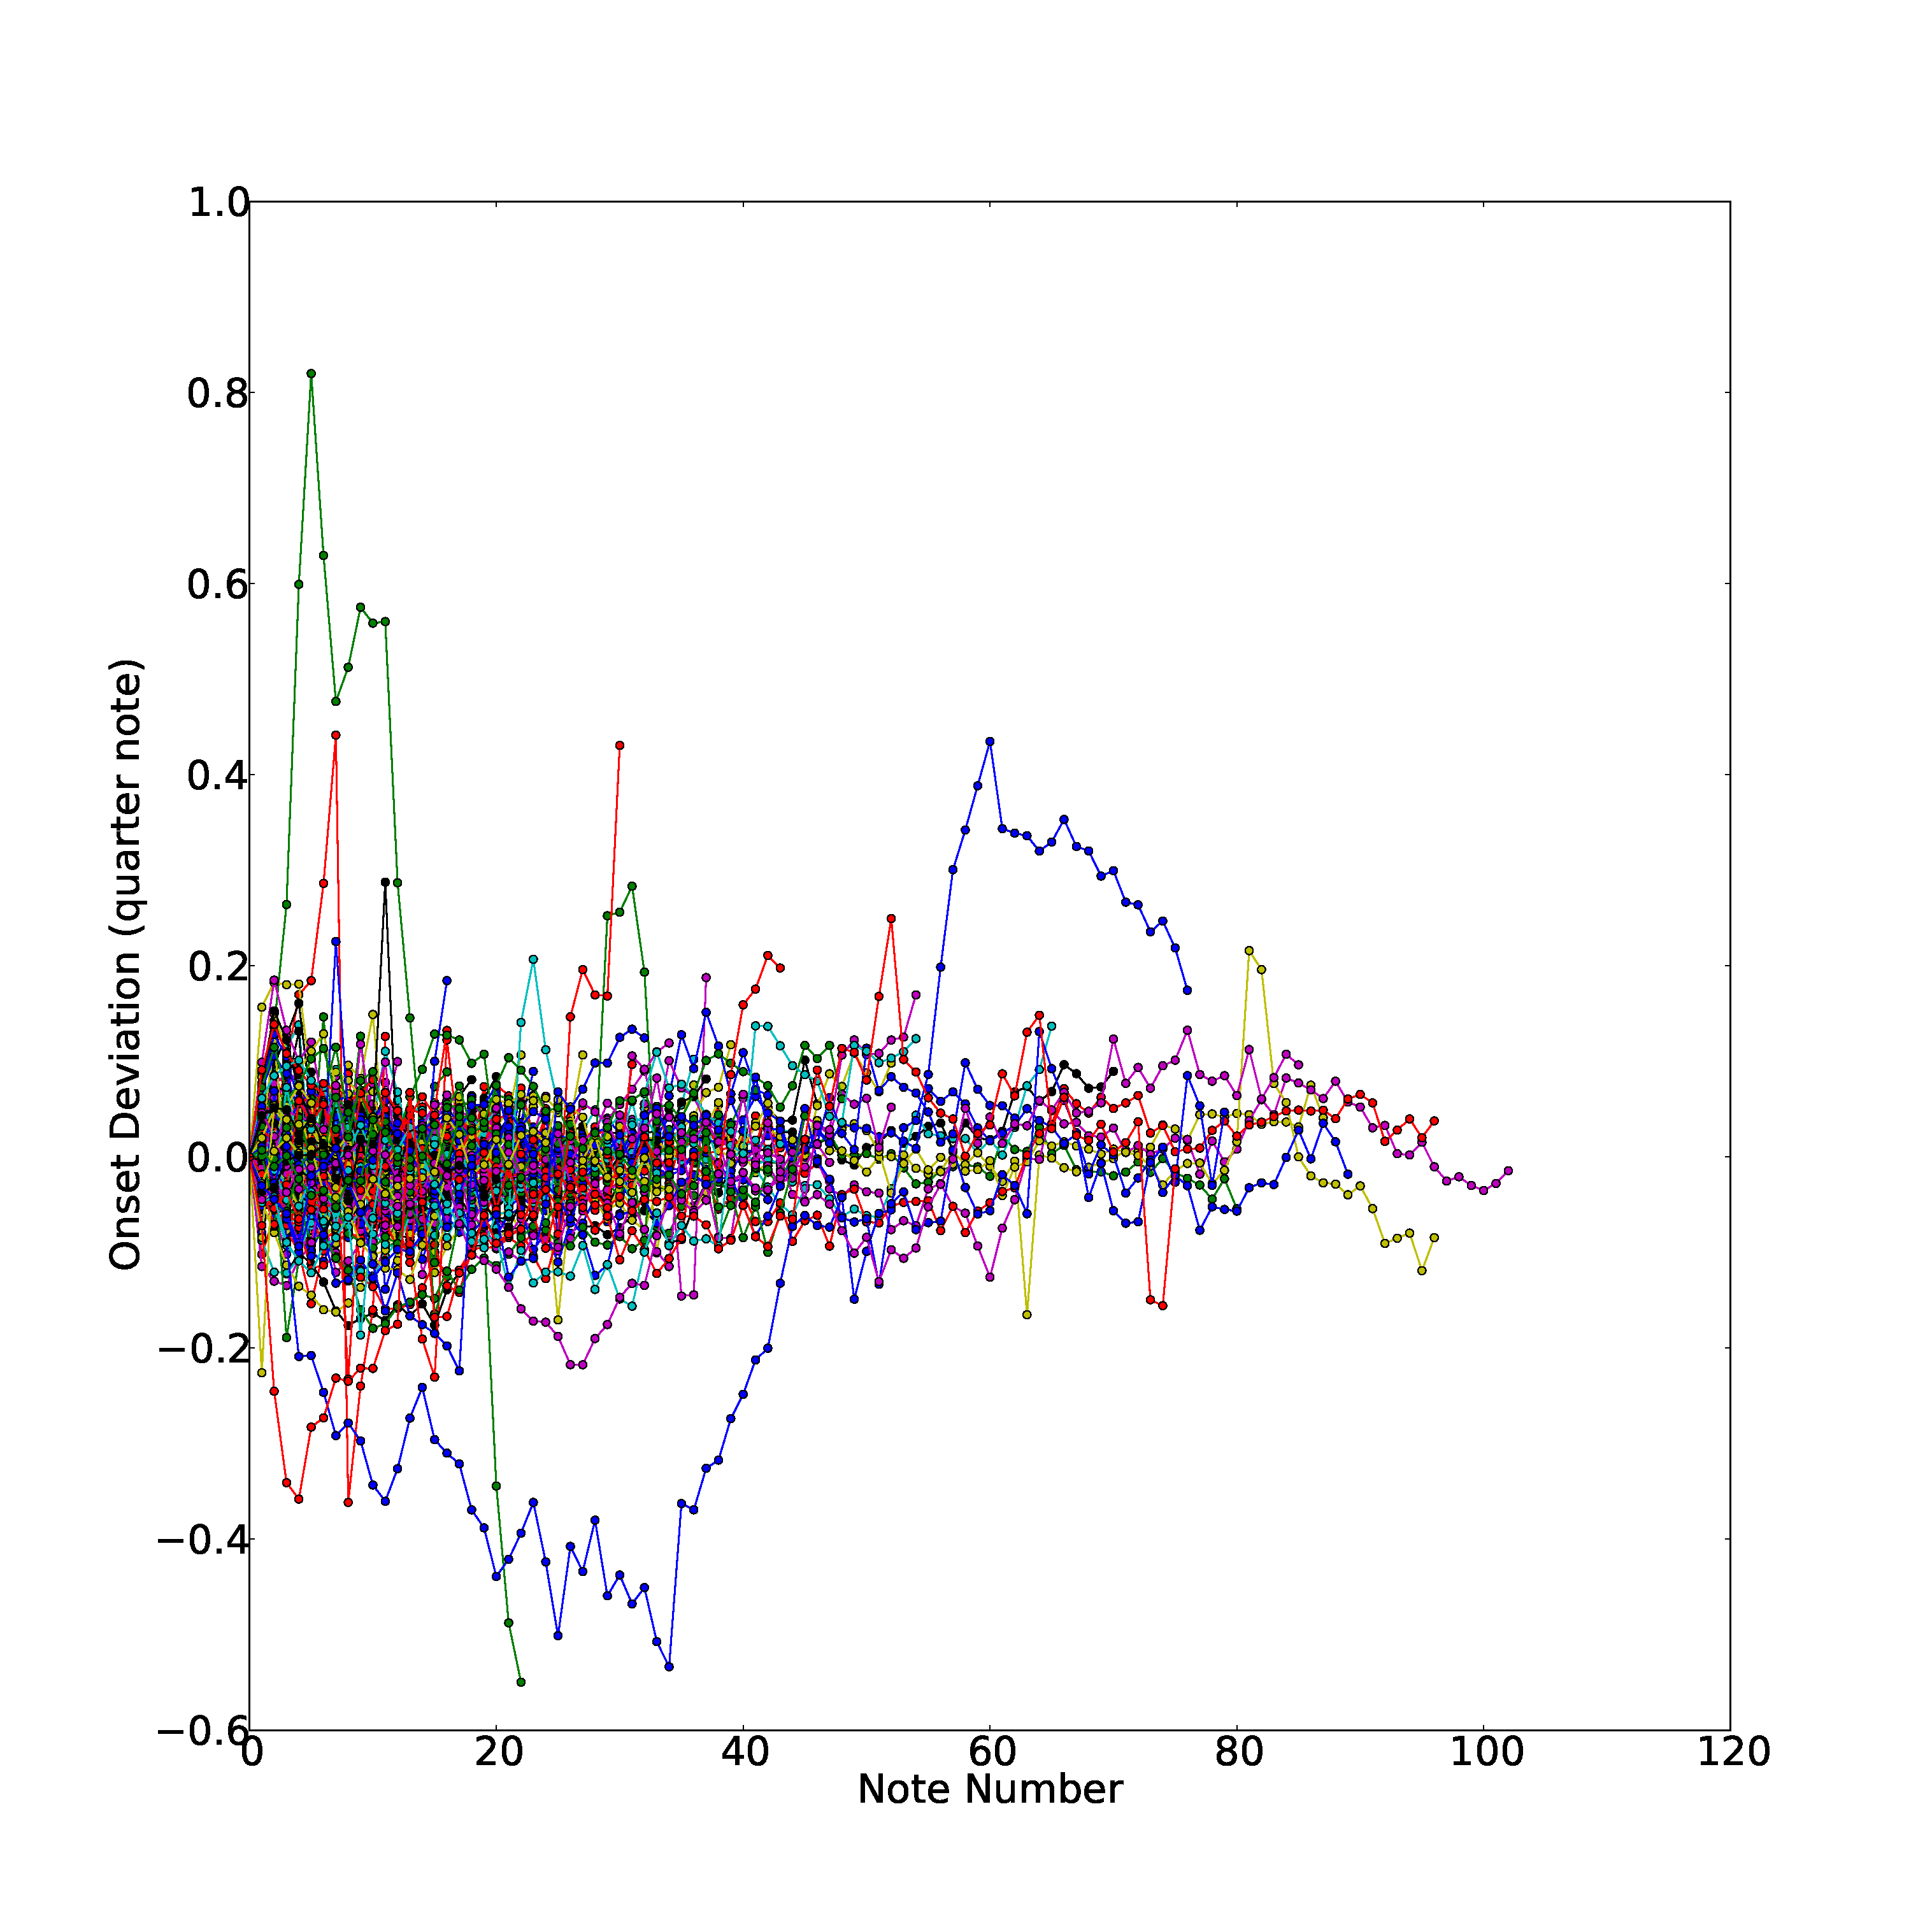
\includegraphics[width=0.6\textwidth]{fig/lian_onset_1}
   \end{center}
   \caption{Onset Deviations Using Auto Normalization Method}
   \label{fig:normauto}
\end{figure}

\begin{figure}[tp]
   \begin{center}
      %TODO:Fig.:Normalization Schemes
      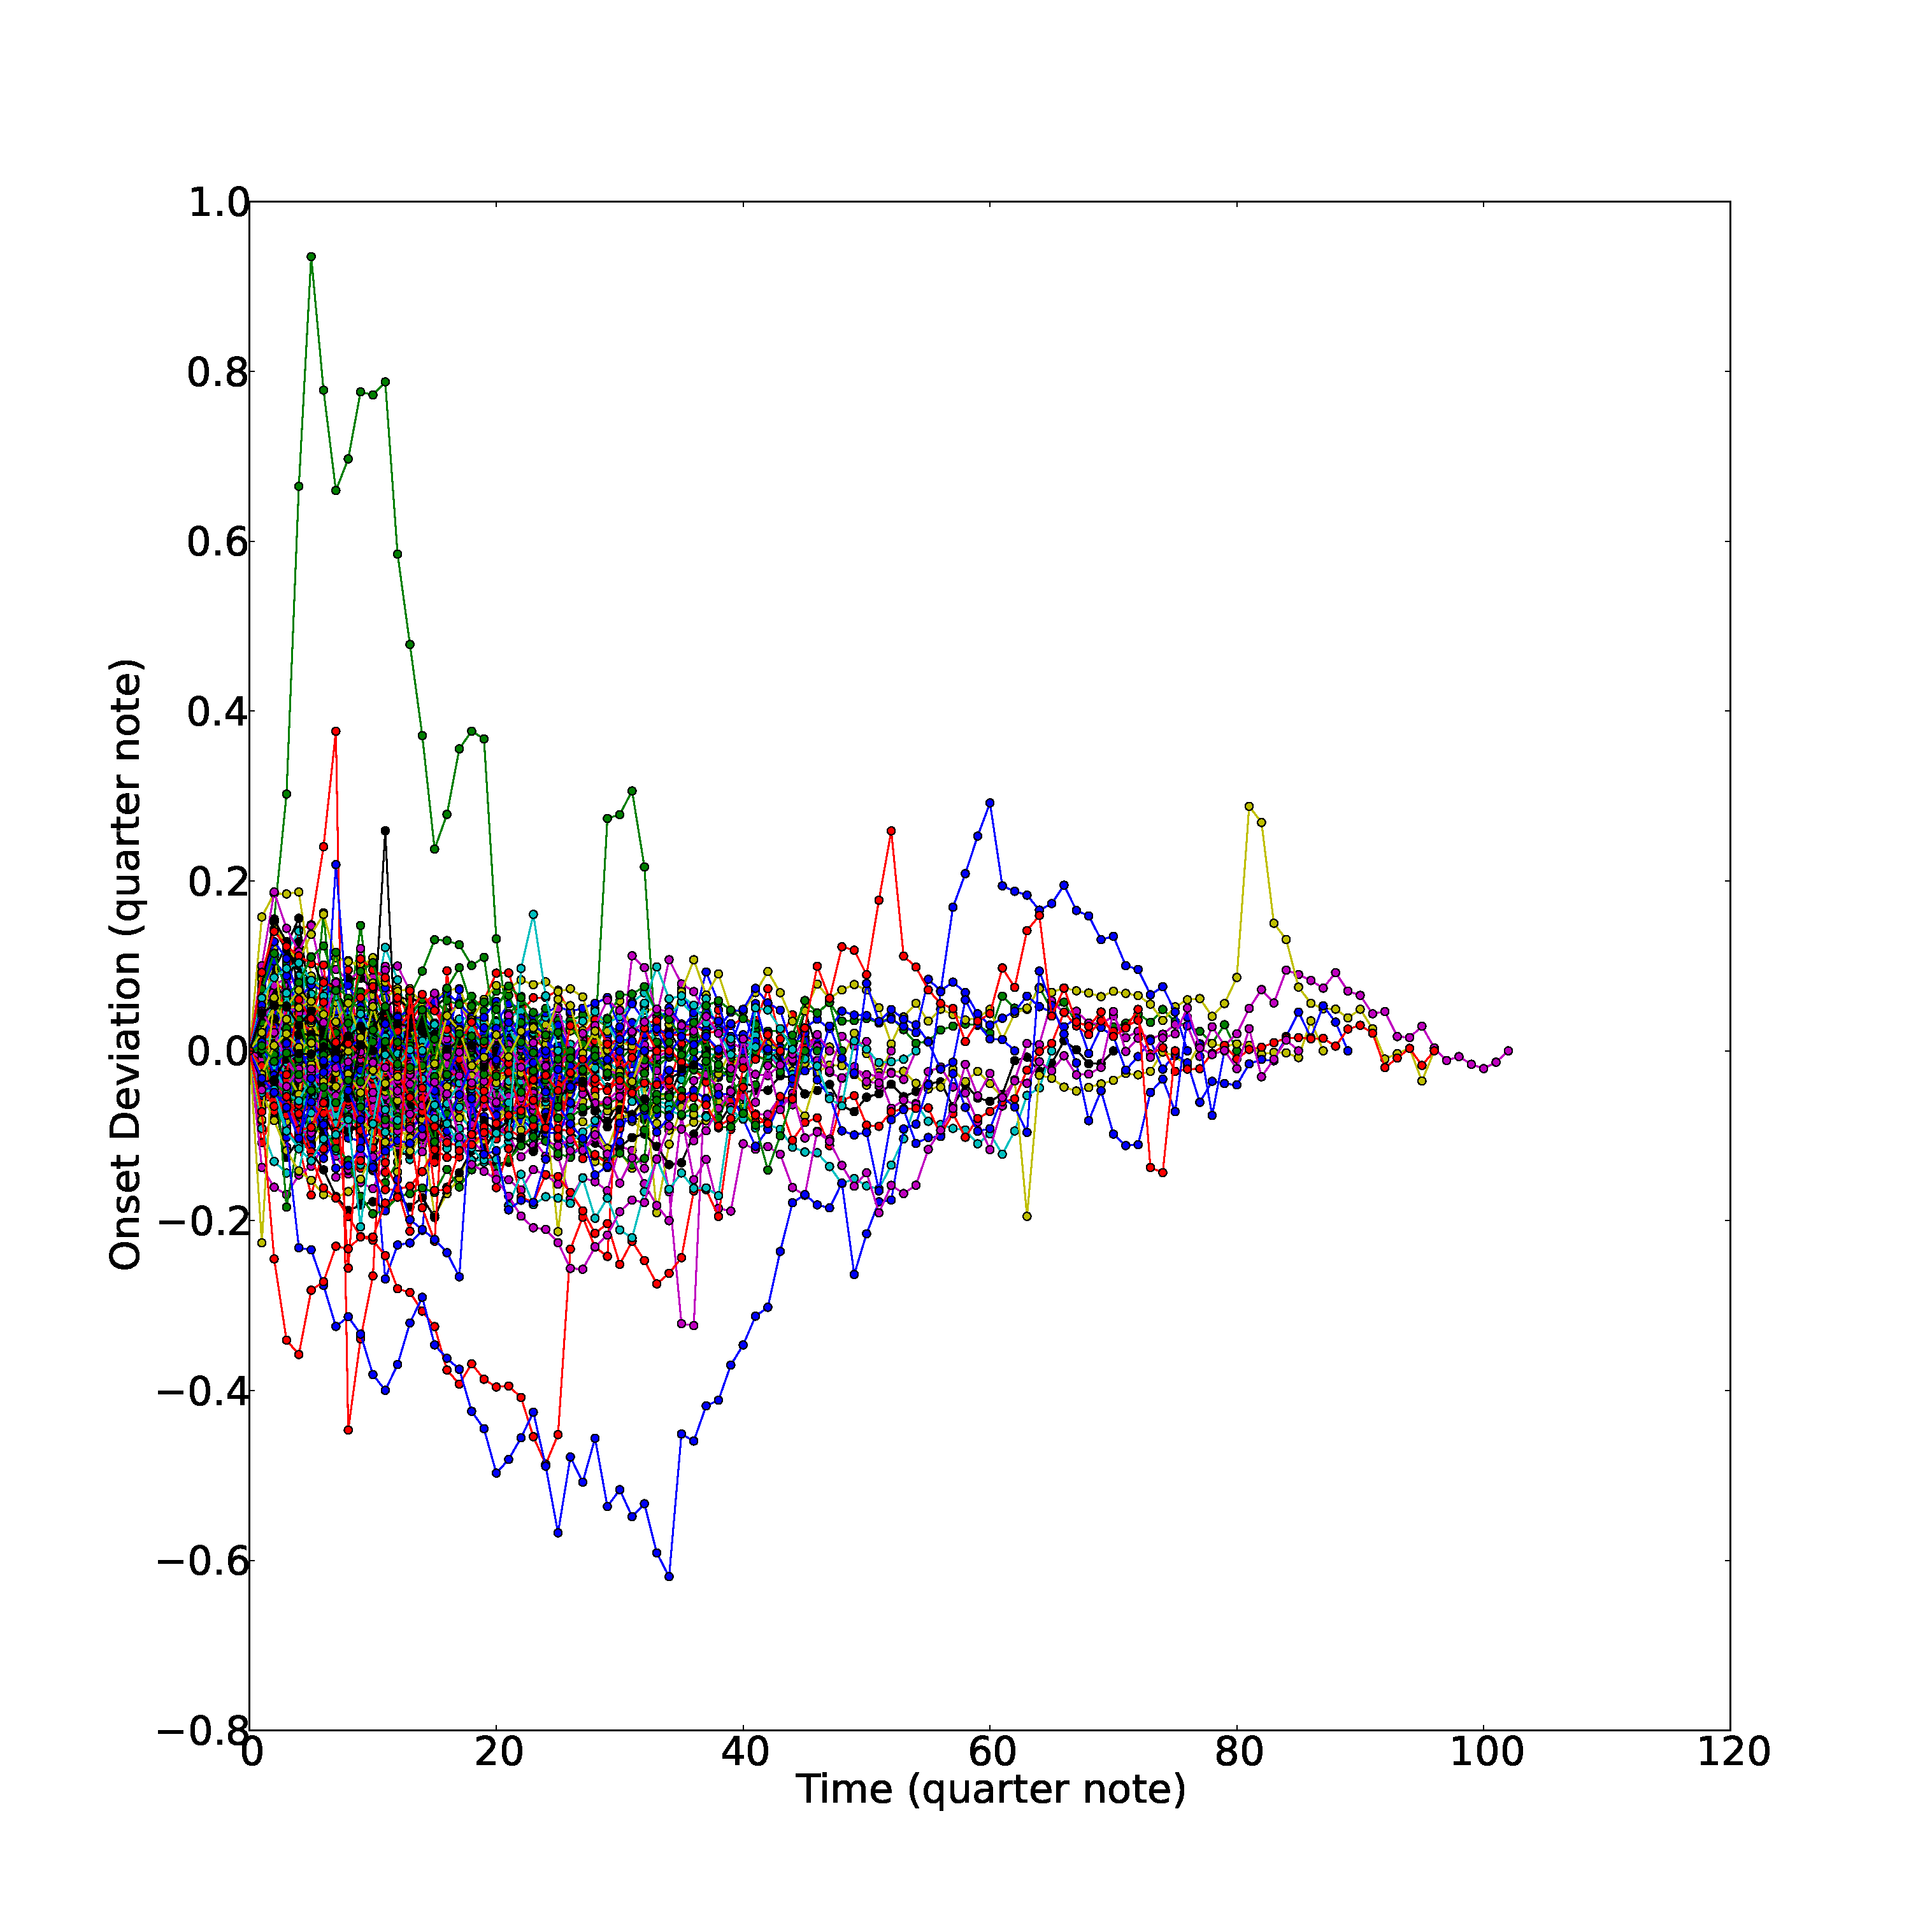
\includegraphics[width=0.6\textwidth]{fig/lian_onset_2}
   \end{center}
   \caption{Onset Deviations By Aligning Last Notes Onset}
   \label{fig:norm1}
\end{figure}

%\begin{figure}[tp]
%   \begin{center}
%      %TODO:Fig.:Normalization Schemes
%      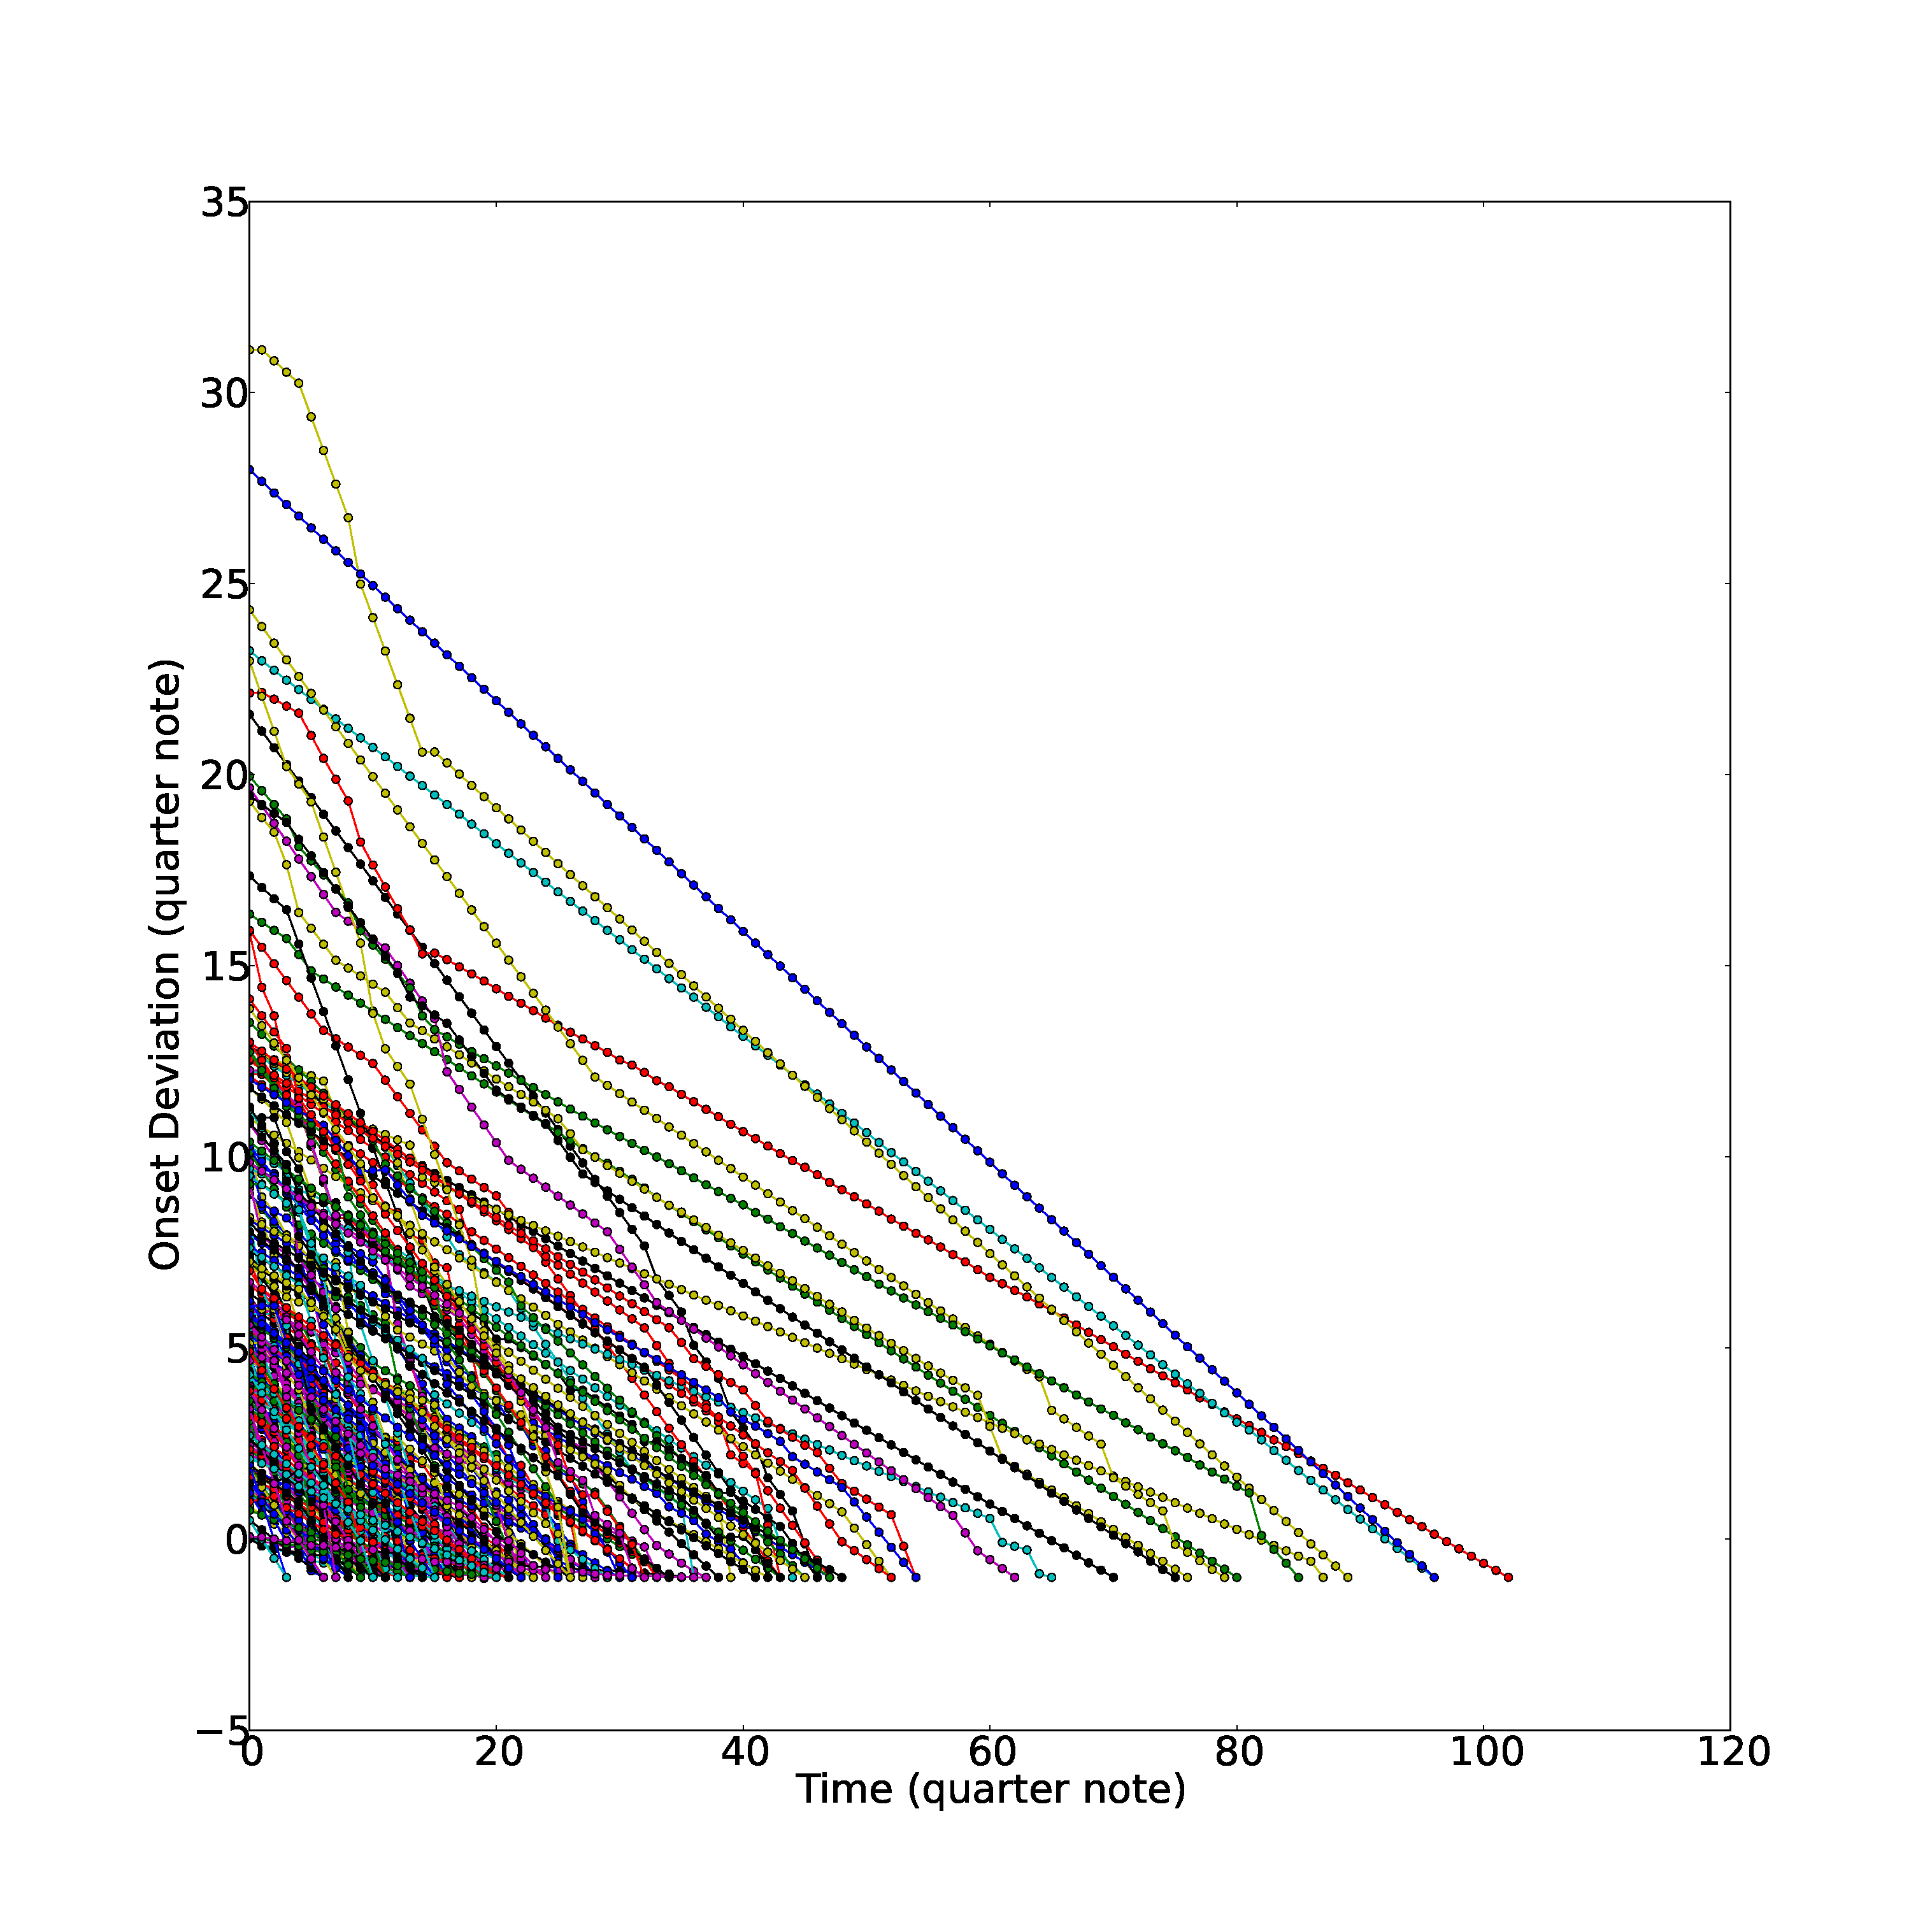
\includegraphics[width=0.6\textwidth]{fig/lian_onset_3}
%   \end{center}
%   \caption{Onset Deviations Using Normalization Method 2}
%   \label{fig:norm2}
%\end{figure}

\begin{figure}[tp]
   \begin{center}
      %TODO:Fig.:Normalization Schemes
      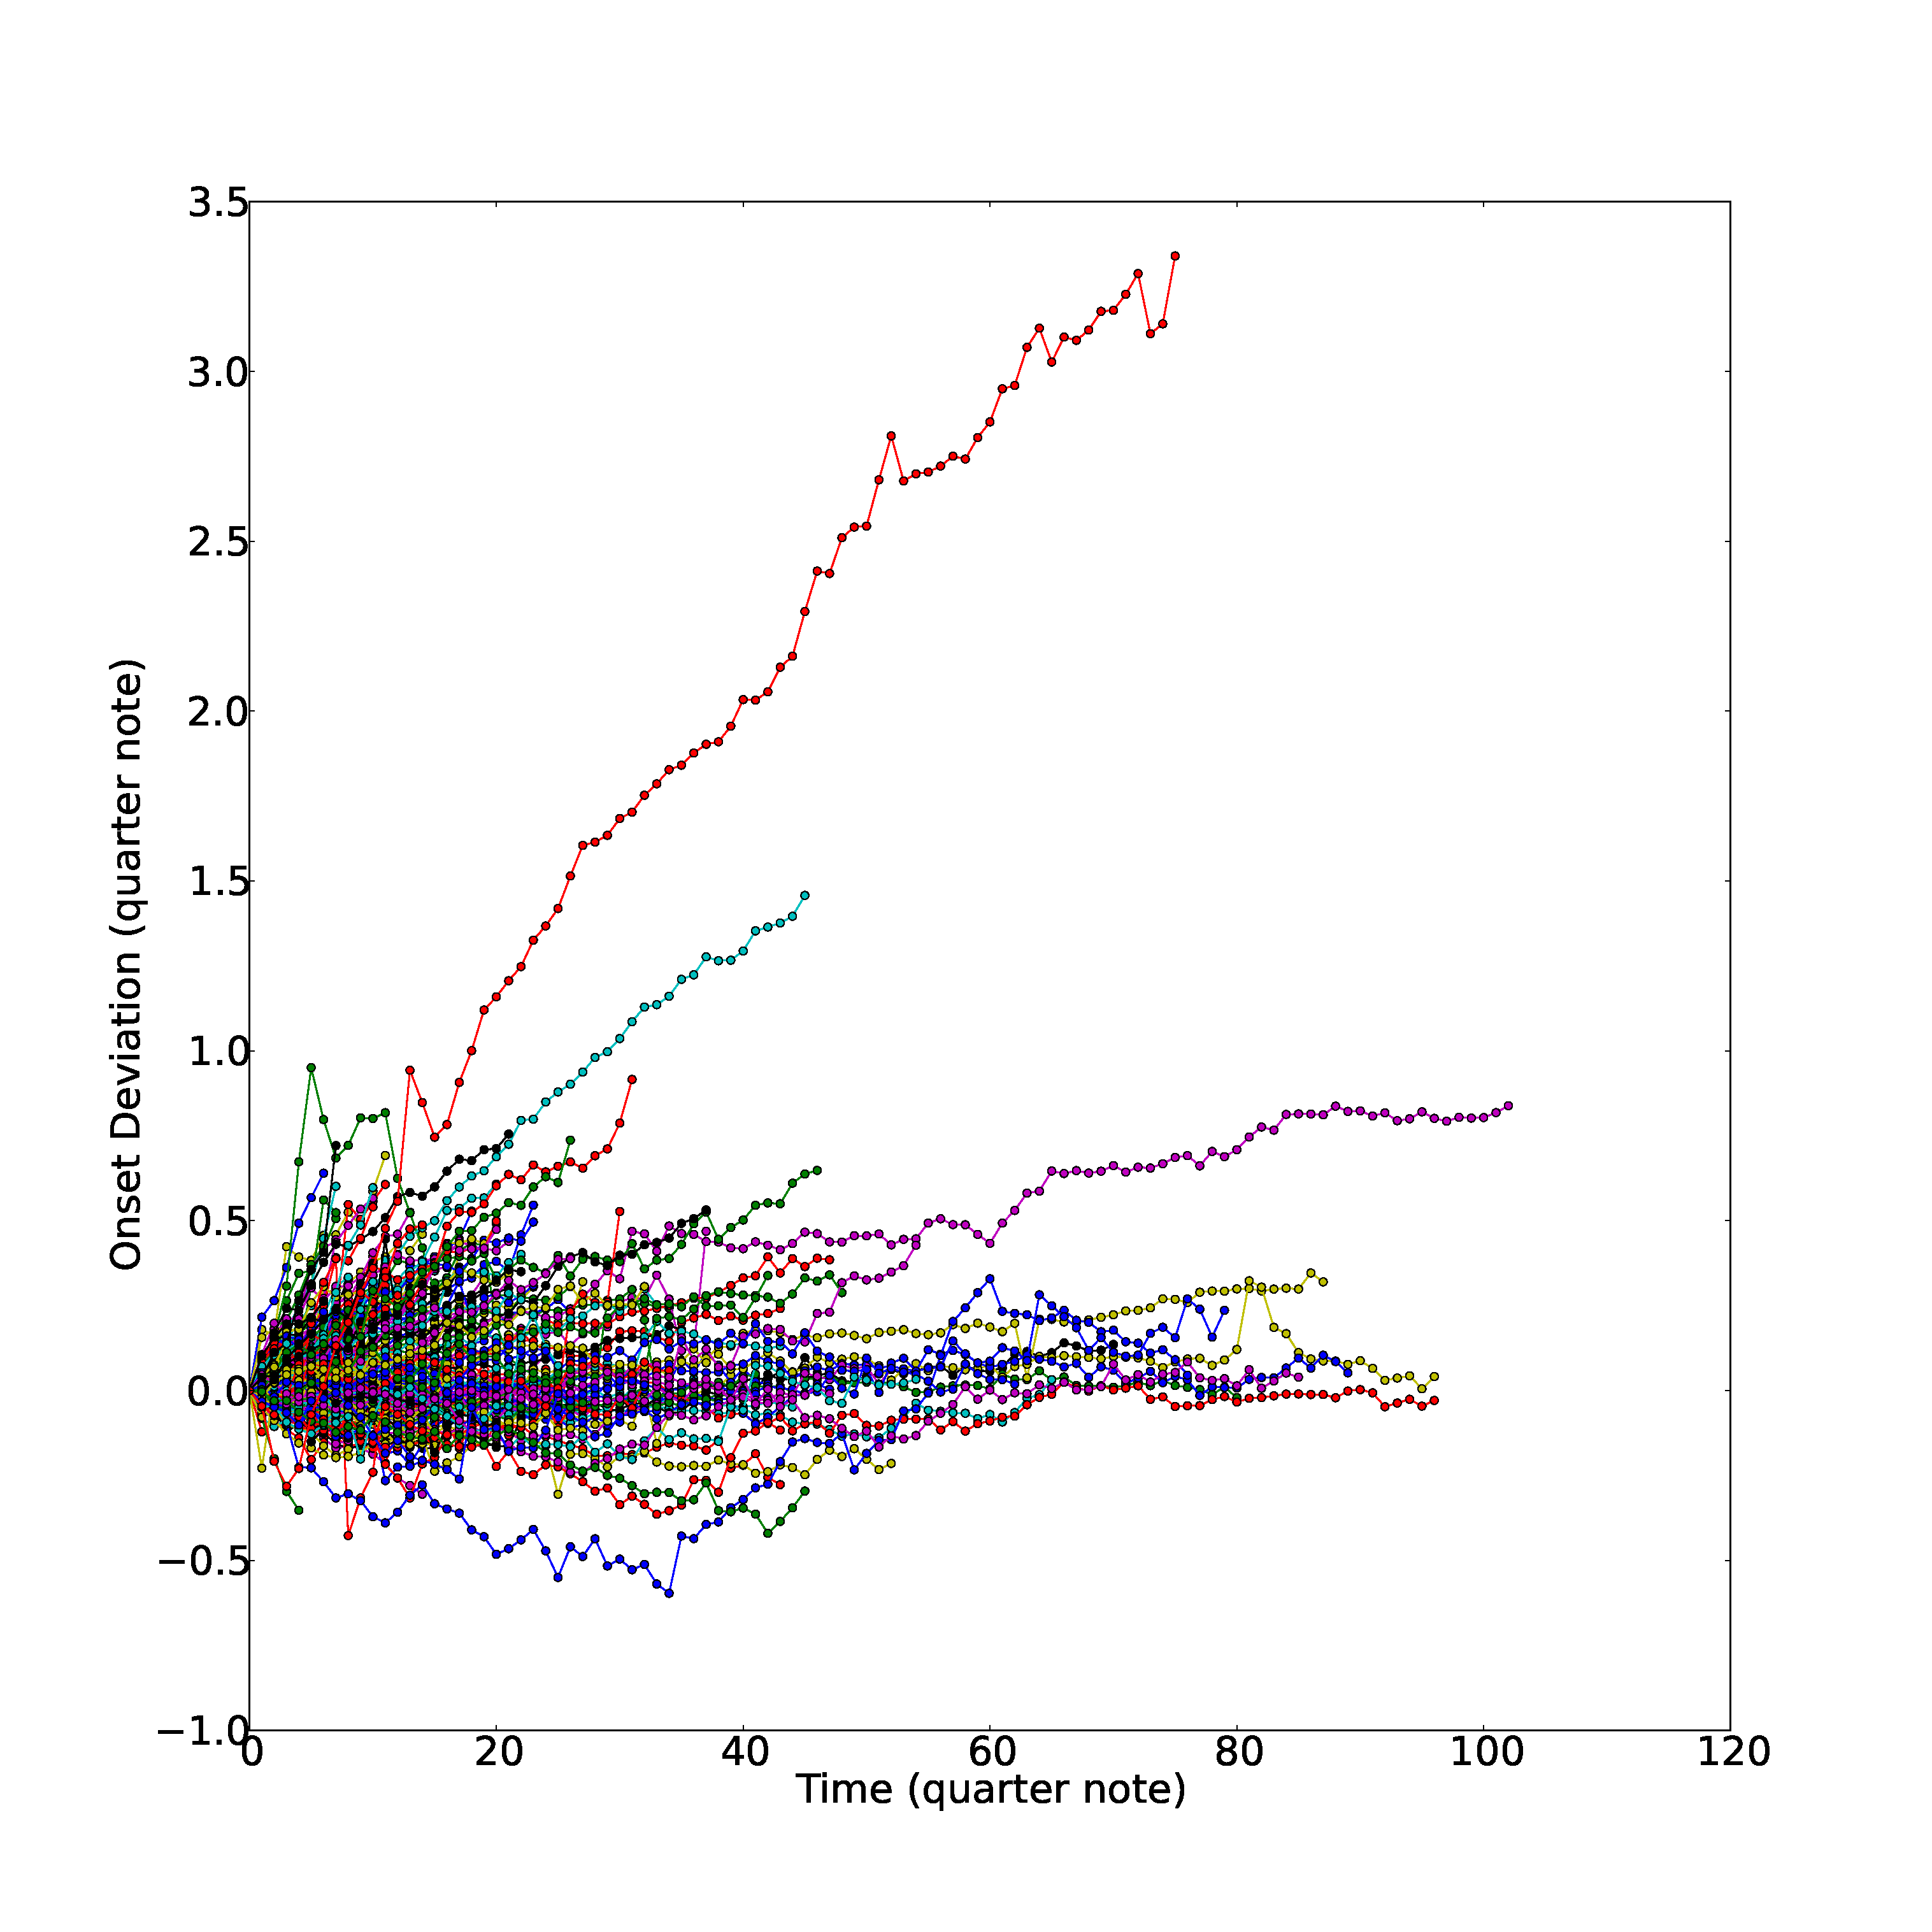
\includegraphics[width=0.6\textwidth]{fig/lian_onset_4}
   \end{center}
   \caption{Onset Deviations By Aligning Last Notes Off}
   \label{fig:norm3}
\end{figure}

%\begin{figure}[tp]
%   \begin{center}
%      %TODO:Fig.:Normalization Schemes
%      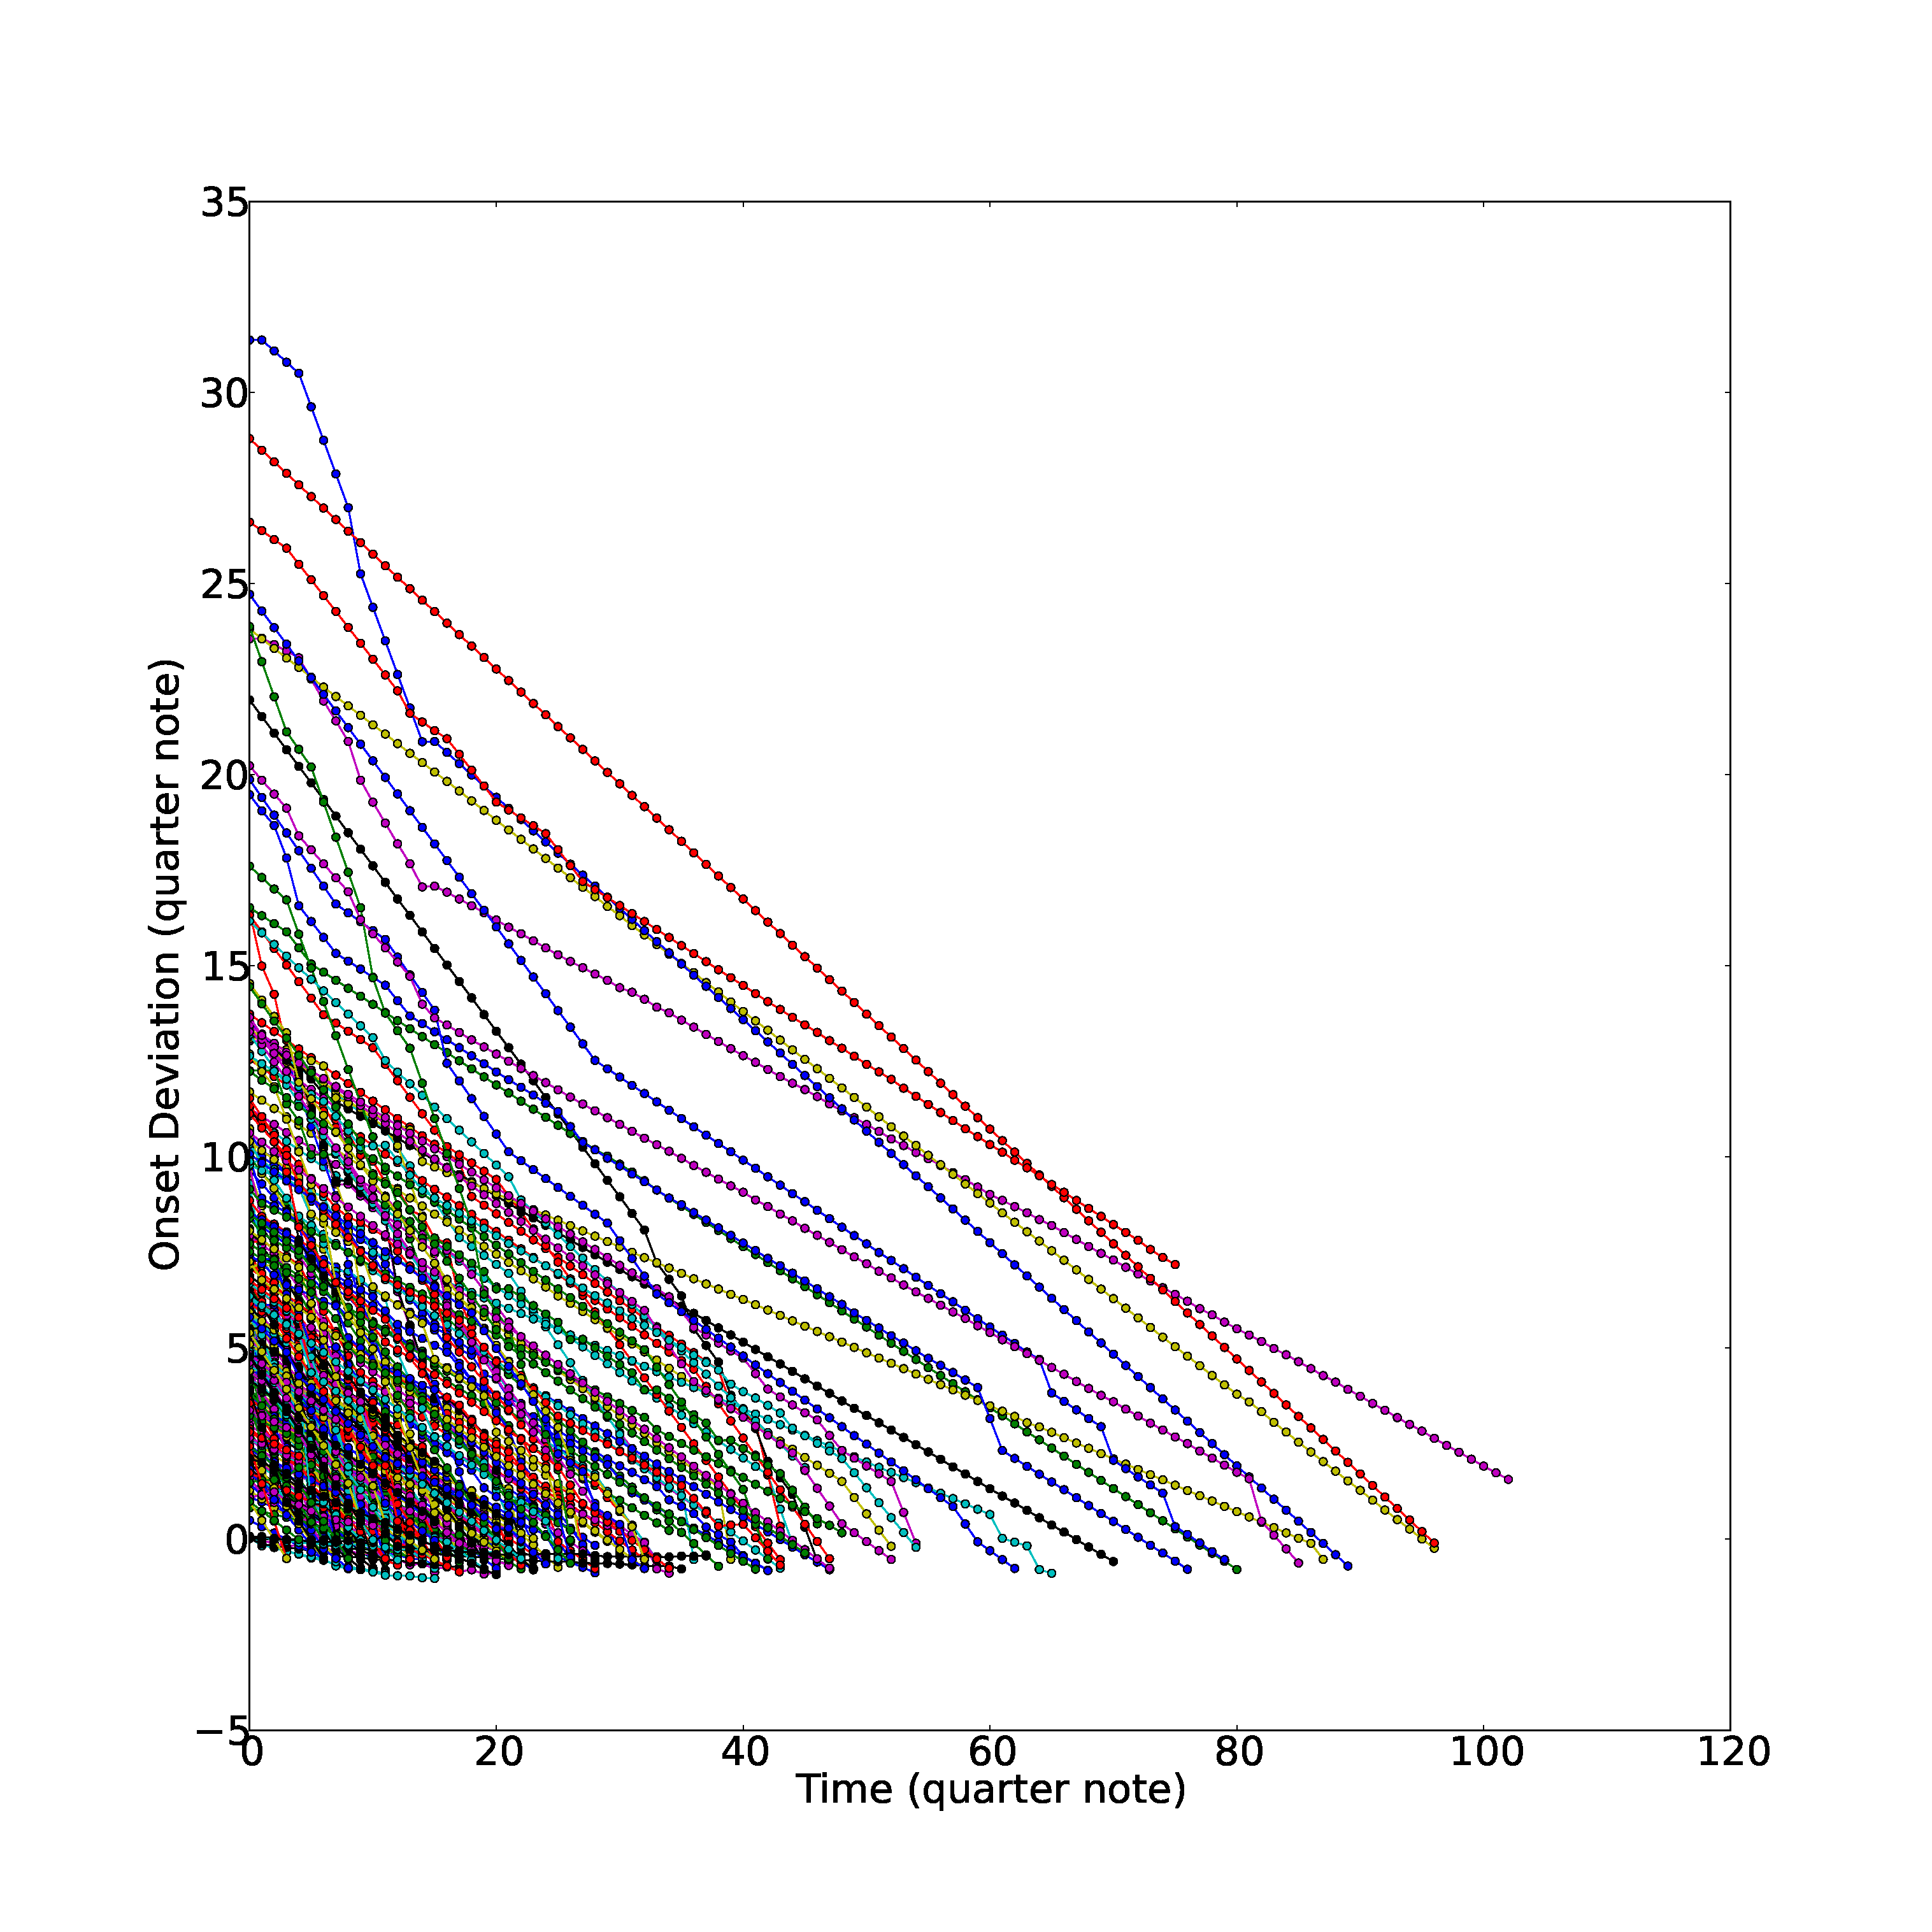
\includegraphics[width=0.6\textwidth]{fig/lian_onset_5}
%   \end{center}
%   \caption{Onset Deviations Using Normalization Method 4}
%   \label{fig:norm4}
%\end{figure}


\section{Parameter Selection}
\label{sec:paramselect}
\subsection{SVM-related Parameters}
Since SVM-HMM is a combination of SVM and HMM, there are many parameters which needs adjustment from both model. Two parameters are tested to find their optimal value: the termination accuracy $\varepsilon$ and the misclassification penalty factor C in SVM. Because the algorithm is an iterative one, the $\varepsilon$ parameter defines the desired accuracy required for the algorithm to terminate. A smaller $\varepsilon$ will result in higher accuracy, but increased execution time (because of more iterations run.) The C parameter determines how hard non-separable samples should be penalised. A large C will sacrifice larger margin for lower misclassification error, but it will make the execution longer.%Therefore, we will leave the rest of the parameters to their default value, and try to find the best C parameter.l

Because it is desirable to generate a performance in a style similar to the training examples, we use the whole set of Clementi's Sonatinas Op.36 from a single performer, and split them into two sets: the training set includes pieces No. 2 to No. 6, and the testing set includes piece No. 1. We train a model with the training set, and use the learned model to generate expressive performance. The computer generated expressive performance should have a similar expression to the testing set. 


%Structural Support Vector Machine has some parameters that needed to be adjusted. We will leave the others to the defaults and change the SVM C trad-off parameter in this experiment. Since three models are learned for three performance features, we have three parameters to adjust. 
%TODO default parameters

%[TODO: phrases count] phrases from [TODO:song counts] songs are used for training. Every first, fifth, and tenth phrases from each song is not included in the training sample, but used as testing samples. A three-by-three grid is layed out for three C parameters, each C takes the value of the powers of tenfrom [TODO: Cs] $10^{-5}$ to $10^4$, so [TODO: num of experiment] paramenters are tested. Then the result is validated
To measure the effectiveness of the $\varepsilon$ and C parameters, the generated performance is compared to the performance recorded by the performer. Ideally, the generated performance will be very similar (in expression) to the recording. So, for every pair of the generated and recorded performances, we calculate their distance, and take the median value of all the distances for every C. Note that each performance feature has its own model, so we will be looking at a single performance feature and its C parameter at a time.  
First, the generated performance features sequence and the recorded one are normalized to a range from 0 to 1. The normalization is required because we want to tolerate linear scaling. Then the Euclidean distance of the two normalized sequence is calculated and divided by the length (in notes) of the phrase, since the phrase can have arbitrary length.


First we will fix C at 0.1 and test different $\varepsilon$'s: 100, 10, 1, 0.75, 0.5 and 0.1. Then, we fix $\varepsilon$ at the optimal value determined in the previous step and test 's: $10^{-3}, 10^{-2}, 10^{-1}, 0.5, 1, 5$, with other parameters set to default. And we will evaluate the optimal parameters and evaluate their execution time. For each $\varepsilon$ or C, we calculate the distance between the generated pieces and recorded examples for all phrases in the testing set for each performer. And we take the median of all these distances for each $\varepsilon$ or C.


%\begin{enumerate}
%	\item Are all the output samples successfully generated? (Generation may fail if the performance features are unreasonable, for example, negative onset timeing.)
%	\item Is the order of the notes preserved? Sometimes the first note is delayed too long and the second note is played too early, so the order is swaped.
%	\item Are there any extreme parameters that makes the expressive performance unnatural?
%\end{enumerate}

%The first two criterias are checked by python scripts, the last one is done by manual inspection.
%
%\framebox{TODO:train / gen corpus}
%\framebox{TODO:how to define distance}
%\framebox{TODO: range of Cs}
%\framebox{TODO: }
%
%\framebox{TODO:experiment result}
%\framebox{TODO: similarity v Cs}
%\framebox{TODO: }
%\framebox{TODO: }
%\framebox{TODO: }
\framebox{TODO: median}
The performance regeneration accuracy for various $\varepsilon$'s are shown in Fig. \ref{fig:eps_accu}. And the time for various $\varepsilon$'s are shown in Fig. \ref{fig:eps_time}. For $\varepsilon$ value 100 and 10, the termination criteria is too generous, so the learning algorithm terminates almost immediately. Therefore, the model hardly learns anything, the output is a fixed value for any input. So we abandon the data points because the model had learned nothing. We can see that the accuracy drops slowly when $\varepsilon$ becomes smaller. But after $\varepsilon$ is smaller than 0.5, the accuracy doesn't drop anymore. So we will choose $\varepsilon = 0.5 $ for the rest of the experiment to avoid unnecessary computations.

\begin{figure*}[tp]
   \begin{center}
      %TODO:Fig.:Example JSON code
      \includegraphics[width=\textwidth]{fig/eps_accu.eps}

   \end{center}
   \caption{Accuracy for Different $\varepsilon$'s}
   \label{fig:eps_accu}
\end{figure*}
\begin{figure*}[tp]
   \begin{center}
      %TODO:Fig.:Example JSON code
      \includegraphics[width=\textwidth]{fig/eps_time.eps}

   \end{center}
   \caption{Execution Time for Different $\varepsilon$'s}
   \label{fig:eps_time}
\end{figure*}

As for different C parameter, the accuracy and execution time are shown in Fig.\ref{fig:c_accu} and Fig. \ref{fig:c_time} respectively. The accuracy forms a U shape curve, with the valley near 0.1. But the execution time grows as C goes larger, so we should choose C = 0.1 as our optimal C.

\begin{figure*}[tp]
   \begin{center}
      %TODO:Fig.:Example JSON code
      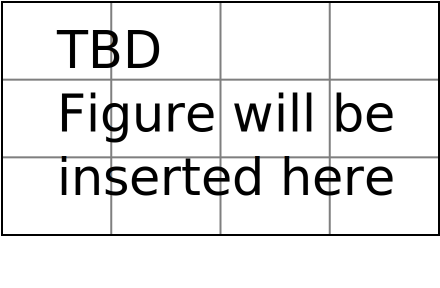
\includegraphics[width=\textwidth]{fig/TBDFigure}

   \end{center}
   \caption{Accuracy for Different C's}
   \label{fig:c_accu}
\end{figure*}
\begin{figure*}[tp]
   \begin{center}
      %TODO:Fig.:Example JSON code
      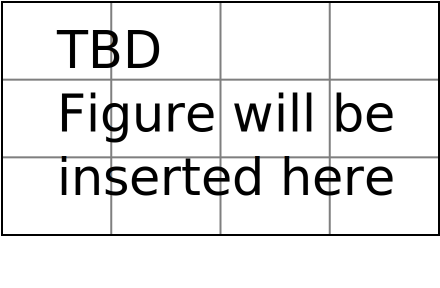
\includegraphics[width=\textwidth]{fig/TBDFigure}

   \end{center}
   \caption{Execution Time for Different C's}
   \label{fig:c_time}
\end{figure*}
\subsection{Quantization Parameter}
Besides $\varepsilon$ and C, the number of quantization levels for SVM-HMM input is also has some impact on the execution time. If the performance features are quantized into more fine-grained levels, the quantization errors can be reduced, but the execution time and memory usage will grow dramatically. Also, larger number of intervals doesn't imply more accurate or robust model. Because SVM-HMM is originally used in part-of-speech tagging problem, if we use divide the performance features into more intervals, than there will be fewer samples for each interval. But it is more desirable that similar phrases will be quantized to the same bin, instead of split them into more fine-grain bins. For example, if a three note segment is played once in the following MIDI velocity: (60, 70, 80), and the same phrase is played again in (60.1, 69.9, 80.1). If we have a quantization interval width of, say, 0.05, then 60 and 60.1 may be quantized into different bins, and 70 and 69.9 may also be quantized to different bins, so the two phrases will be considered as two different case. However, if the quantization interval width is 1, both phrases may be the same after quantization, which is more desirable because the SVM-HMM algorithm can capture the similarity in the two samples. 

Initially, we tried to quantized the values into 1025 uniform width bins, wishing to minimize quantization error. But it take very long time to learn a model. So we switch to a more reasonable value: 128. From empirical data, onset deviation feature rarely exceeds $\pm 1$, so the quantization interval is around $\frac{1-(-1)}{128} = 0.015625$. Most duration ratios falls between zero and three, so the interval is $\frac{3-0}{128} = 0.0234375$. And MIDI velocity is around 30 to 90, so the interval is about $\frac{90-30}{128} = 0.46875$. This level of granularity is good enough for our performance system, and can dramatically reduce the execution time without sacrificing the expressiveness of the models. 

We repeat the $\varepsilon$ selection experiment in the previous section for quantization level of 1025 and 128. The execution time (in CPU second) is shown in Fig. \ref{fig:quant_comp}. The time required for 1025 is larger than 128 by orders of magnitudes. The outcome, however, is still expressive, as can be heard in the Section \ref{sec:turing}.

\begin{figure}[tp]
   \begin{center}
      %TODO:Fig.:Normalization Schemes
      \includegraphics[width=\textwidth]{fig/quant_comp}
   \end{center}
   \caption{Execution Time for different Quantization Granularity}
   \label{fig:quant_comp}
\end{figure}

\section{Human-like Performance}
\label{sec:turing}
The most general purpose of a expressive performance system is to create expressive, non-robotic music as oppose to deadpan MIDI. Therefore, we would like to perform a Turing-test-style survey to find out how people think about the our generated expressive music.

In this survey, 1518 computer generated expressive phrases and their corresponding human recording are used as candidates. Each test subject was given 10 randomly selected computer generated phrase and 10 random human recordings, the 20 phrases are presented in random order. He/She was asked to evaluate each phrase according to the following criteria, which are proposed by RenCon contest\cite{rencon}:
\begin{enumerate}
   \item Technical control – if a performance sounds like it is technically skilled thus performed with accurate and secure notes, rhythms, tempo and articulation.
   \item  Humanness – if the performance sounds like a human was playing it.
   \item  Musicality – how musical the performance is in terms of tone and color, phrasing, flow, mood and emotions
   \item Expressive variation – how much expressive variation (versus deadpan) there is in the performance.
\end{enumerate}

In RenCon, each judge is asked to give separate ratings for each criteria. But we believe that the understanding the difference between the four criteria and give separate rating is too demanding for less-experienced participant, so we asked test subjects to vote an overall rating from one to five. One being very bad, five being very good. The test subject are also asked to report their musical proficiency in a three level scale:
\begin{enumerate}
   \item No experience in music 
   \item Amateur performer
   \item Professional musician, musicologist or student majored in music
\end{enumerate}

To generate the expressive performance phrase. We follow a six-fold cross validation pattern. For each performer in the corpus, we use all his/her recorded phrase from Clementi's Op.36 No. 2 to No. 6 to train a model. Then the model is used to generate all phrases from Clementi's Op.36 No. 1. The generate phrases and the performer's recording of piece No. 1 will all be included into the test set. \framebox{Maybe we should compare to other people's recording?} The process is repeated, but this time we use pieces No. 1, 3, 4, 5, 6 to train a model, and generate piece No. 2, and so on. So all six pieces will have a computer generated version and recorded version for each player's corpus.

%With these music material ready, we built a survey web page to let the test subjects vote. A test subject was first asked to report their music proficiency (No music training at all, amateur or professional musician/scholar/student) and musical instrument skill. Then he/she will be asked to identify the computer generated phrase from a generated/recorded pair. Five pairs will be randomly selected from all the available pairs, and the order of appearance of the generated and recorded one will be randomized.

We have also tried to use all performer's recording instead of just one person's corpus to generate models. However, the expressive variation from the model is much smaller than a single performer's model. This is because the expression from different performer may cancel out each other. The distribution of each performance features are presented in Fig. \ref{fig:distonset} to Fig. \ref{fig:distvel}. For each performance feature, the frequency of occurrence of different feature values are counted and plotted as histograms. The features generated from the full corpus are more concentrated, which results in less dramatic expression.


\begin{figure}[tp]
   \begin{center}
      %TODO:Fig.:Normalization Schemes
      \includegraphics[width=0.6\textwidth]{fig/all_01_onset}
   \end{center}
   \caption{Distribution of Onset Deviation Values from Full Corpus versus Single Performer's Corpus}
   \label{fig:distonset}
\end{figure}
\begin{figure}[tp]
   \begin{center}
      %TODO:Fig.:Normalization Schemes
      \includegraphics[width=0.6\textwidth]{fig/all_01_duration}
   \end{center}
   \caption{Distribution of Duration Ratio Values from Full Corpus versus Single Performer's Corpus}
   \label{fig:distdur}
\end{figure}
\begin{figure}[tp]
   \begin{center}
      %TODO:Fig.:Normalization Schemes
      \includegraphics[width=0.6\textwidth]{fig/all_01_velocity}
   \end{center}
   \caption{Distribution of MIDI Velocity Values from Full Corpus versus Single Performer's Corpus}
   \label{fig:distvel}
\end{figure}


\framebox{TODO:Turing test result and discussion}

%We distributed a web survey to check if our computer generated performance are indistinguishable to human recordings.  The expressive performance generated by the method described above are collected, as well as all human recordings from the corpus. Each participant will be given ten random phrases from the computer generated phrases, and ten random phrases from human recordings. The twenty phrases will be presented in random order. The participant are asked to give 

We received 119 valid samples from the survey. Fifty of them are from people with no music background, 59 are from amateur musicians, and the rest 10 are from professional musicians. The average rating given to computer generated performance and human recordings are listed in Table \ref{tab:avg_rating}. It is clear that for professional and amateur musician, the average rating given to human performances are higher than computer performances. However, for participants who have no experience in music, the rating is much closer. A Student T-test on the two ratings for participants with no experience yields a p-value of 0.0312, therefore we can't reject the null hypothesis that the two ratings are different under a significance level of 99\%.

\begin{table}
   \centering
   \caption{Average Rating for Generated Performance and Human Recording}
   \label{tab:avg_rating}
   \begin{tabular}{r|rr}
      \hline
      &Computer &Human \\
      \hline
      No experience&3.243&3.391\\
      Amateur&2.798&3.289\\
      Professional&2.430&3.010\\
      \hline
      Total&2.952&3.306\\
      \hline
   \end{tabular}
\end{table}

In order to get more insight from the ratings, we can further divide the performers in the corpus in to two categories based on their piano skill. By the number of mistakes made (Table \ref{tab:mistakes}), performer A and B are considered more skilled, and performer C, D, E and F are considered less skilled. The average rating given to the two categories are listed in Table \ref{tab:good-bad_rating}. The distance between computer and human performances are smaller for less skilled group (C to F) than the more skilled group (A and B). This is probably because our system makes some mistakes that are similar to the mistakes made by less-skilled performers. For example, unsteady tempo, sudden change in loudness, hesitation and emphasising notes that are structurally less important are all common problems that exists in both less-skilled performance and computer generated performance. But for more-skilled performer, because of they have better technical control and sense of musical structure, the problems described above will happen less often. %This is probably because our system still can't capture every nuance of human performances.

\begin{table}
   \centering
   \caption{Average Rating for Generated Performance and Human Recording under Different Part of the corpus}
   \label{tab:good-bad_rating}
   \begin{tabular}{r|rr|rr}
\hline
&A,B&&C-F&\\
&Computer &Human &Computer &Human \\
\hline
No experience&3.067&3.302&3.363&3.451\\
Amateur&2.680&3.347&2.863&3.286\\
Professional&2.048&3.162&2.708&2.921\\
\hline
Total&2.776&3.313&3.066&3.323\\
\hline
   \end{tabular}
\end{table}

If we look into each individual participant, we can see if a participant gives higher (average) rating to computer or human performances, or equal ratings. The number of participants who fall into each categories are shown in Table \ref{tab:avg_count}. Twenty-six non-experienced participants give higher or equal rating to computer than human, slightly higher than twenty-four people who gives higher rating to human. For amateur and professional musicians, the number of people who prefers human are much higher. Table \ref{tab:good-bad_count} is a table similar to \ref{tab:avg_count}, but split into two categories just like Table \ref{tab:good-bad_rating}. The results are similar to Table \ref{tab:avg_count}: the difference between computer and human is higher for skilled performers (A and B) than less-skilled performers (C to F).


\begin{table}
   \centering
   \caption{Number of Participants Who Gives Higher Rating to Generated Performance, Human Recordings or Equal Rating}
   \label{tab:avg_count}
   \begin{tabular}{r|rrr|r}
      \hline
      &Computer&Equal&Human&Total\\
      \hline
      No experience&19&7&24&50\\
      Amateur&7&3&49&59\\
      Professional&1&1&8&10\\
      \hline
      Total&27&11&81&119\\
      \hline
   \end{tabular}
\end{table}

\begin{table}
   \centering
   \caption{Number of Participants Who Gives Higher Rating to Generated Performance, Human Recordings or Equal Rating under Different Part of the Corpus}
   \label{tab:good-bad_count}
   \begin{tabular}{r|rrr|rrr|r}
\hline
&&A,B&&&C-F&&Total\\
&Computer&Equal&Human&Computer&Equal&Human&\\
      \hline
No experience&5&4&6&14&3&18&50\\
Amateur&2&1&18&5&2&31&59\\
Professional&0&1&3&1&0&5&10\\
      \hline
Total Result&7&6&27&20&5&54&119\\
      \hline
   \end{tabular}
\end{table}
